%% ============================================================================================
%% DRAFT v2, part 2: Methodology (study design).  No results in this section.
%% ============================================================================================

\section{Methodology}
\label{sec:design}

\begin{figure}[t]
\centering
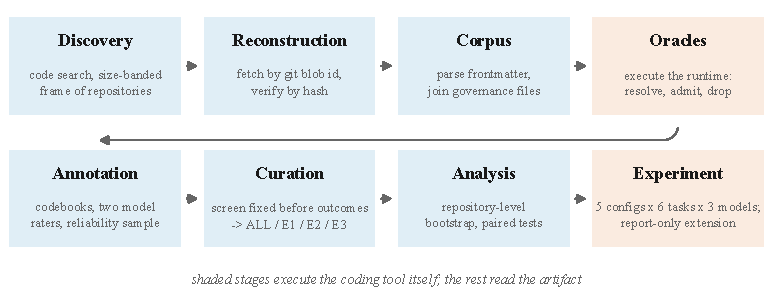
\includegraphics[width=\textwidth]{fig0_pipeline}
\caption{The study pipeline. Two stages execute the coding tool itself: the oracles, which establish what the
runtime resolves and admits, and the experiment, which establishes what agents do under a given grant. Every other
stage reads the artifact.}
\label{fig:pipeline}
\end{figure}

Figure~\ref{fig:pipeline} shows the pipeline. The correspondence with the ACM SIGSOFT repository-mining standard
\citep{ralph2021empirical} and the LLM guidelines \citep{baltes2026guidelines} is given in the replication package.

%% ---------------------------------------------------------------------------
\subsection{Data collection}
\label{sec:collection}

\paragraph{Discovery.} GitHub code search is the only public index of file contents; it returns at most 1,000 results
per query, considers only the default branch, and may return incomplete results when a query times out
\citep{GitHubSearchAPIDoc}. We partitioned the query \code{path:.claude/agents extension:md} into 28 file-size bands and
used the results only to discover repository names (27--28 August 2026), yielding a frame of \nFrame{} repositories. The
original run's per-band log was not archived. In a same-day re-run, all \nBandsTruncated{} bands reported more matches
than the interface serves (\nReportedTotal{} files in total), and the re-run found \nRerun{} repositories, including
\pctRerunOverlap{} of the frame. The frame is therefore about \pctFrameOfRerun{} of the repositories the re-run found,
selected by GitHub's undocumented relevance ranking, and because discovery is file-level, repositories with many agent
files had more chances to be found. Our results describe this frame; we make no inference to all public
repositories.

\paragraph{Inventory and snapshot-exact reconstruction.} For each frame repository one Git Trees API call returned its
complete file listing with the git blob identifier of every file (five listings were truncated and are reported). We
kept agent definitions and the co-located settings files, \code{.mcp.json} files and CI workflows. Each file was then
fetched \emph{by its blob identifier} rather than from a moving branch head, and verified by recomputing its git object
hash, so every file is the snapshot's version and every failed request is visible. Table~\ref{tab:coverage} reports
coverage; the \nFilesUnavailable{} files that could not be fetched are kept in the corpus with their status.

\begin{table}[t]
\caption{Reconstruction coverage. Files were fetched by git blob identifier and verified by recomputing the object
hash, so a recovered file is the snapshot's byte content rather than a later state of the path.}
\label{tab:coverage}
\footnotesize
\begin{tabular}{@{}>{\raggedright\arraybackslash}p{7.0cm}r@{}}
\toprule
\textbf{Stage} & \textbf{Count} \\
\midrule
Repositories in the discovery frame & \nFrame{} \\
Agent-definition files inventoried & \nInventoryFiles{} \\
Files recovered and hash-verified & \nFilesOk{} \\
Files unavailable (repository inaccessible or object missing) & \nFilesUnavailable{} (\pctUnavailable{}) \\
\midrule
Subagent specifications in the corpus & \nSpecsAll{} \\
Repositories contributing at least one specification & \nReposAll{} \\
Engineered repositories (E2) / their specifications & \nReposEng{} / \nSpecsEng{} \\
\midrule
Distinct \code{tools}/\code{disallowedTools} combinations probed by the resolver oracle & \nDistinctGrants{} \\
Distinct tool names probed individually & \nDistinctNames{} \\
Configuration roots probed by the census oracle & \nRootsCensus{} \\
Released versions probed for the tool pool & \nReleasesHistory{} \\
\bottomrule
\end{tabular}
\end{table}


\paragraph{Repository metadata.} For every frame repository we collected repository flags, dates, contributors,
licence, languages, the README, governance files and settings (\S\ref{sec:governance}) and monthly commit counts up to
the snapshot; contributors and protection state are observable only as of collection (15--16 September 2026).

%% ---------------------------------------------------------------------------
\subsection{Data curation}
\label{sec:curation}

The unit of observation is a \emph{specification}: a file under a \code{.claude/agents/} directory whose frontmatter
parses and declares \code{name} and \code{description}, the runtime's own admission rule (validated in
\S\ref{sec:oracles}). The unit of analysis is the repository. Table~\ref{tab:perils} maps the perils of mining GitHub
\citep{kalliamvakou2016promises}, and the threats specific to code-search discovery, to how this study addresses each.
The central one is that many repositories are personal, inactive or not software. Following the structure of Galster et al.'s curation \citep{Galster2026Dataset}, a metadata screen followed by README
classification, we fixed a curation protocol in writing before joining any outcome to repository metadata
(\code{annotation/engineered\_filter\_protocol.md}). Their thresholds (at least 352 commits and 18 months of age) would
remove \pctGalsterReposRemoved{} of the specification-bearing repositories, since the format dates from mid-2025, so we
adapted them:

\begin{description}\itemsep1pt
  \item[Stage A (metadata)] A1 not a fork, archived, disabled, template, mirror or empty repository; A2 at least 50
        commits on the default branch before the snapshot; A3 commits in at least three distinct months; A4 at least
        one commit in the six months before the snapshot; A5 at least 10\,kB of source code detected by GitHub Linguist.
  \item[Stage B (README classification)] Each repository is classified from its name, description, topics, languages,
        activity counts and README (codebook P) into \emph{engineered}, \emph{template collection}, \emph{tutorial or
        learning}, \emph{personal configuration}, \emph{demo or experiment}, \emph{non-software} or \emph{unclear}.
\end{description}

We analyse four nested populations (Table~\ref{tab:populations}): \textbf{ALL} specification-bearing repositories;
\textbf{E1}, those passing Stage A; \textbf{E2}, those also classified as engineered, the \emph{primary population};
and \textbf{E3}, E2 restricted to repositories with at least two contributors and a licence, the closest analogue of
Galster et al.'s criteria. The grant-type, dominated-withholding and mode-gap quantities are reported under all four
populations and on one copy per content hash; the language samples (\S\ref{sec:nlp}) are drawn from E2 only. The
protocol also pre-declared silent-defect rates and prose--grant consistency under all four populations; these are
reported for E2 only, a deviation from the protocol.

\begin{table}[t]
\caption{Threats from mining GitHub that bear on this study: perils of \citet{kalliamvakou2016promises} (Roman
numerals give their number) and threats specific to code-search discovery (marked $\dagger$,
\citealp{GitHubSearchAPIDoc}), what each would do to our conclusions, and the mitigation applied.}
\label{tab:perils}
\footnotesize
\begin{tabular}{@{}>{\raggedright\arraybackslash}p{2.8cm}>{\raggedright\arraybackslash}p{3.9cm}>{\raggedright\arraybackslash}p{4.3cm}@{}}
\toprule
\textbf{Peril} & \textbf{Threat to this study} & \textbf{Mitigation} \\
\midrule
Personal or inactive repositories (III, V) & Prevalences would describe scratch repositories &
Screen fixed in a written protocol before outcomes were joined; four nested populations
(\S\ref{sec:curation}) \\
Not software projects (IV) & Tutorials, dotfiles and prompt collections counted as engineering practice &
Stage~B excludes every repository not classified as engineered \\
A repository is not a project (I) & Mono-repositories inflate team size & Repository is the unit of analysis \\
Activity is uneven (II) & Repositories with many specifications dominate pooled statistics & Prevalences are means of
within-repository proportions unless labelled pooled \\
Forks and branches not indexed ($\dagger$) & The frame misses copies and non-default-branch work & Stated as a
limitation \\
Search incomplete and unstable ($\dagger$) & All bands truncated; the frame is about \pctFrameOfRerun{} of the
repositories found, chosen by an undocumented ranking & Size-banded queries, re-run the same day (covers
\pctRerunOverlap{} of the frame); results describe the frame; shares checked by repository size \\
Repositories change (XIII) & Later edits contaminate a ``snapshot'' & Files fetched by blob identifier, verified by hash \\
Duplication ($\dagger$, this study) & Repositories are not independent & One-copy-per-hash sensitivity analysis
(\S\ref{sec:threats}) \\
Not only on GitHub (VI) & Mirrors carry stale or partial state & Mirrors excluded (A1) \\
Pull requests, users (VIII, IX, XI) & Merge- or user-activity measures mislead & Not applicable (commit-based activity) \\
\bottomrule
\end{tabular}
\end{table}

\begin{table}[t]
\caption{The engineered-project screen, fixed in a written protocol before outcomes were joined
(\S\ref{sec:curation}). Stage~A is metadata only; Stage~B adds the README classification. The grant, dominance and
mode-gap results are reported under ALL, E1, E2 and E3.}
\label{tab:populations}
\footnotesize
\begin{tabular}{@{}l>{\raggedright\arraybackslash}p{5.6cm}rr@{}}
\toprule
\textbf{Population} & \textbf{Screen} & \textbf{Repositories} & \textbf{Specifications} \\
\midrule
ALL & every repository contributing a specification & 4{,}128 & 69{,}316 \\
\quad A1 & not a fork, archive, template, mirror or empty repository & 4{,}019 & 67{,}697 \\
\quad + A2 & at least 50 commits to the snapshot & 2{,}581 & 39{,}734 \\
\quad + A3 & at least 3 months with a commit & 1{,}969 & 29{,}866 \\
\quad + A4 & a commit within six months of the snapshot & 1{,}861 & 28{,}041 \\
E1 & + A5: at least 10\,kB of source detected by Linguist & 1{,}852 & 27{,}901 \\
E2 & + README classified as an engineered software project & 1{,}508 & 21{,}116 \\
E3 & + at least two contributors and a licence & 887 & 11{,}303 \\
\bottomrule
\end{tabular}
\end{table}


%% ---------------------------------------------------------------------------
\subsection{Parsing schema and capability model}
\label{sec:parsing}
\label{sec:capmodel}

\paragraph{Grant types and effective grant.} Each specification is parsed into the fields of Table~\ref{tab:schema},
with its \emph{configuration root} (the directory holding \code{.claude/}) and body text. A specification makes an \textbf{explicit grant} when it declares a
\code{tools} list and an \textbf{implicit grant} when it omits the field and so inherits the tool pool. The two are
reported separately. The tools a specification can use are not the tools it
lists: its \textbf{effective grant} $G(s)$ is the tool set observed by the resolver oracle (\S\ref{sec:oracles}) after
resolving \code{tools} and \code{disallowedTools}, plus any requested credential-gated tools the credential-free oracle
cannot see. A specification \textbf{can write files} if $G(s) \cap \{\code{Write}, \code{Edit},
\code{NotebookEdit}\} \neq \emptyset$ and \textbf{can run a shell} if $G(s)$ contains \code{Bash} or \code{Monitor}
(\code{PowerShell} resolves only on Windows and is not observable on our macOS oracle). A shell is \textbf{scoped} when
every shell entry the author wrote carries a command pattern such as \code{Bash(git diff:*)}. The resolver reports a
scoped entry as \code{Bash}. The documentation describes such patterns for permission rules in settings, and says
that a Bash deny rule applies to subagents, but does not say whether a pattern in a subagent's \code{tools} field is enforced when the subagent calls
the shell \citep{AnthropicSubagentsDoc,AnthropicPermissionsDoc}. We tested it (\S\ref{sec:res-rq3}): in auto
permission mode on v\ScopedBuild{}, a subagent granted \code{Bash(git log:*)} ran arbitrary shell commands. We
nevertheless count scoped shells as non-dominating, which makes every dominance and prose--grant measure a lower
bound; the scoped share is small (\RQthreeScopedShare{} of write-withholding grants that keep a shell).

\paragraph{Dominance.} Following Miller's distinction \citep[\S8.1]{miller2006robust}, let $\mathrm{reach}(t)$ be the
set of effects an agent can bring about through tool $t$, directly or through programs it can launch. Tool $t$
\textbf{dominates} tool $u$ if $\mathrm{reach}(t) \supseteq \mathrm{reach}(u)$. An unsandboxed, unscoped shell
dominates every file tool, because any file operation can be issued as a command. A specification exhibits a
\textbf{dominated withholding} when its effective grant withholds every file-writing tool but contains an unscoped
shell. The term describes the grant, not the author's intent: some such specifications are meant to change files
through the shell (\S\ref{sec:res-rq3}). The experiment (\S\ref{sec:experiment}) tests dominance by execution.

\paragraph{Execution context and threat model.} Whether a shell command runs is also decided outside the
specification. The parent session's permission mode sets what runs without asking \citep{AnthropicPermissionModesDoc}:
in \code{default} mode only reads, so every other shell command needs the user's approval; in \code{acceptEdits} also
file edits and common file-system commands; in \code{auto} everything, with background safety checks by a classifier;
in \code{dontAsk} only pre-approved tools, and anything else is denied; in \code{bypassPermissions} everything. Under
\code{auto}, \code{acceptEdits} and \code{bypassPermissions} a subagent runs in the parent's mode and its own
\code{permissionMode} is ignored; otherwise its own mode applies \citep{AnthropicSubagentsDoc}. Allow and deny rules,
hooks and a sandbox can further permit or block a command. A dominated withholding therefore has no effect on what the
delegate can write when shell commands run without per-command approval (\code{auto}, \code{bypassPermissions},
\code{acceptEdits} for common file-system commands, or an allow rule covering the shell) and without a sandbox; in
\code{default} mode the user's approval of each command is the control, and in \code{dontAsk} such commands are
denied. The session's mode and user-level settings are not observable in a repository, so we measure the grant and
report the committed context (\S\ref{sec:res-rq3}). The asset we consider is the integrity of the
repository's files; the threat is a change the configuration was meant to prevent, requested by a parent that
misjudges the task or by content the delegate reads. The capability model covers file integrity through
built-in tools only. It does not cover network egress (e.g.\ \code{WebFetch}), tools from MCP servers, further
delegation or the confidentiality of what an agent reads, so our estimates of authority are lower bounds on what
agents can do, not upper bounds.

%% ---------------------------------------------------------------------------
\subsection{Executable oracles}
\label{sec:oracles}

\paragraph{Observation point.} In print mode with streaming JSON output, Claude Code emits a start-up record, before
contacting the model, that lists the resolved tools and registered agents; started as a named agent (\code{--agent}),
the tool list is that agent's effective grant. Each oracle stages the files under test in a fresh directory and starts
the pinned build (v2.1.233, macOS arm64) with an empty configuration directory, so no credential, settings, plugins or
MCP servers are loaded and the process exits when its first request fails to authenticate.

\paragraph{Oracles.} The \emph{census oracle} stages all agent files of every configuration root at their original
relative paths and reads back the registered agents, which yields the specifications admitted, the files not admitted
and names that collapse. The \emph{resolver oracle} stages every distinct combination of \code{tools} and
\code{disallowedTools} values (\nDistinctGrants{}) and reads its effective grant; every distinct non-MCP tool name
(\nDistinctNames{}) is also resolved on its own, separating names the runtime does not resolve from names dropped only
in combination. The \emph{settings oracle} stages each committed \code{.claude/settings.json}; the settings layer prints
one warning per deny or ask rule that matches no known tool. \emph{Semantics probes} established the behaviours in
Table~\ref{tab:schema}; the same-root precedence probes were repeated three times with the same winner, the others run
once. The default tool pool of
\nReleasesHistory{} releases between May 2025 and September 2026 was recorded in the same way, dating when each name
entered and left the vocabulary, and for every specification naming a removed tool we retrieved the date of the
earliest default-branch commit touching the file.

\paragraph{Oracle validity.} (i) Some tools are enabled by server-side flags fetched only with a credential; in
authenticated probes, nine tools resolved that the credential-free oracle does not see. None of them writes files; one,
\code{Monitor}, runs a shell command and is counted as a shell. Names in that set are not counted as unresolved.
(ii) Interactive-only tools cannot be observed in print mode; they are classified from the build's tool schema as
context-conditional rather than unresolved. (iii) The oracles observe registration and resolution, not behaviour.

%% ---------------------------------------------------------------------------
\subsection{Annotation with LLMs}
\label{sec:annotation}

Six annotation tasks use language models, following \citet{baltes2026guidelines}: role and intended mode (codebook R),
engineered status of repositories (P), topics of directive sentences (C), the write restriction a whole specification
states (S), the use its text makes of a retained shell (B) and completion claims in experiment answers (K). Codebook R
was piloted on 400 items, revised once (v1.1; the changes are recorded in the codebook) and frozen; codebooks P and C
(v1.0) were used unrevised, as were S, K and B.

\paragraph{Codebook R.} Each unique pair of \code{name} and \code{description} (\nRoleItems{} items covering all
\nSpecsAll{} specifications; the annotator does not see the body) receives a \emph{role} from sixteen categories grounded in software-engineering activities
and multi-agent role taxonomies \citep{he2025lmase}, and an \emph{intended mode}: \emph{inspect} if the stated purpose
can be fulfilled without creating, modifying or deleting files or running state-changing commands, \emph{change} if it
requires them, \emph{mixed} or \emph{unclear}. The mode, not the role, is the construct against which least privilege
is judged. The annotator also records whether the description claims read-only status.

\paragraph{Protocol.} Each annotator is a Claude subagent restricted to reading the codebook and one batch file and
writing its labels, with no shell; outputs are validated and missing or invalid items re-annotated. The primary annotator for
codebooks R, P, C, S and B is Claude Haiku~4.5 (\code{claude-haiku-4-5-20251001}); codebook K, which judges a few
hundred short answers, uses Claude Sonnet~5 (\code{claude-sonnet-5}). Random reliability samples of role items
(\nReliabilityItems{}) and of codebook-S and codebook-B specifications are re-annotated independently by Sonnet in
different batch compositions, and Krippendorff's $\alpha$ is reported with the thresholds of
\citet{krippendorff2018content}. Sonnet also labelled 400 role items (under R v1.0) and 450 constraint sentences during
the pilot; these pilot items keep Sonnet's labels, and Haiku labels every other item. Codebook P was applied by Haiku
alone, a deviation from the protocol, which named Sonnet as primary rater and planned a second-rater sample; README
agreement is estimated from the human sample. For human validation, two authors independently code a sample of
\nHumanSample{} items with the codebooks and texts the models saw (\code{annotation/human\_v2}): 200 role items
(codebook R), 80 specifications under codebook S, 60 under codebook B and 60 repositories under codebook P, each
stratified by the primary rater's label. \authornote{Report human--human and consensus--model $\alpha$ per codebook
here, from \code{code/human\_agreement.py}.}

%% ---------------------------------------------------------------------------
\subsection{Language analysis of descriptions and bodies}
\label{sec:nlp}

\paragraph{Directive sentences.} After fenced code is removed, each Latin-script body sentence is tagged with the
strongest deontic marker it contains, with levels modelled on RFC~2119 \citep{rfc2119}: prohibition (\emph{never},
\emph{must not}, \emph{do not}, and also \emph{should not}, \emph{cannot}, \emph{does not} and \emph{avoid}, which alone
mark \pctProhibitionWeakOnly{} of prohibition sentences), obligation (\emph{must}, \emph{always}, \ldots),
recommendation or permission; prohibitions and obligations are \emph{directive}. The lexicon is published. A random
sample of \nConstraintSample{} of the \nDistinctDirective{} distinct directive sentences, stratified by modality, was
annotated with codebook C for its topic and whether it restricts the agent's own writes.

\paragraph{Prose restriction of a specification (codebook S).} Whether a text restricts the agent's own writes is a
property of the whole text (``you are a reviewer; report findings to the parent agent'' forbids nothing lexically). We
drew one specification at random from each engineered repository (\nSpecSample{}) and
annotated its name, description and body: \emph{full} if the text makes the agent read-only, \emph{partial} if it
forbids or conditions some writes, \emph{none} otherwise, with a verbatim quote as evidence. The annotator does not see
the \code{tools} field; bodies over 40{,}000 characters are shown as their first 30{,}000 and last 10{,}000. \nSpecReliabilityBatches{} of
the \nSpecBatches{} batches (\nSpecReliability{} specifications; whole batches, so a cluster sample) were annotated
independently by the second rater. A fully read-only
specification is \textbf{inconsistent} if its effective grant can still reach the file system, through a file-writing
tool or an unscoped shell. With one specification per repository, sample shares estimate repository-level prevalence.

\paragraph{What a retained shell is for (codebook B).} To test whether a dominated withholding keeps a shell the
specification needs, we drew one specification at random from each engineered repository that contains one (explicit
grant, no file-writing tool, unscoped shell; \nShellSample{} specifications) and coded the most state-changing use of a
shell its text asks for or clearly implies: \emph{change} (create, modify or delete files, or change repository,
environment or external state, e.g.\ install, format, commit), \emph{verify} (build, test, lint or run the program
without being asked to change anything), \emph{inspect} (only read or query state, e.g.\ \code{git log}, \code{grep})
or \emph{none} (the text never mentions running commands). The annotator does not see the \code{tools} field. Sonnet
annotated \nShellReliabilityBatches{} batches (\nShellReliability{} specifications) independently.


%% ---------------------------------------------------------------------------
\subsection{Controlled execution experiment}
\label{sec:experiment}

\paragraph{Design.} Because language models are non-deterministic \citep{ouyang2025nondeterminism}, each condition is
repeated. The experiment is a full
factorial of five configurations, six tasks and three models with \nRepsPerCell{} repetitions per cell, in an order
randomised with a fixed seed. The configurations are \textbf{C0} no restriction (no \code{tools}, neutral prompt),
\textbf{C1} prompt restriction only (no \code{tools}; the prompt forbids creating, modifying or deleting files and
running file-changing commands), \textbf{C2} tool restriction only (\code{tools: Read, Grep, Glob, Bash}, the modal
inspection grant), \textbf{C3} both, and \textbf{C4} tool restriction without a shell (\code{tools: Read, Grep, Glob}).
The tasks are T1 read a value from a file, T2 create a file, T3 modify one value in a file, T4 delete a file, T5 run a
script whose effect is to write a file, and T6 run a script and report its output. T2--T5 are forbidden by the prompt of
C1 and C3; T1 and T6 are permitted everywhere, and T6 needs a shell. The models are Claude Haiku~4.5, Sonnet~5 and
Opus~5.

\paragraph{Execution.} Each run is a real delegation: an orchestrating Claude Code session (desktop app, \code{auto}
permission mode, in which shell commands run without per-command approval, subject to the classifier) dispatches a project subagent whose frontmatter carries the configuration's \code{tools} value and
whose body is the configuration's prompt, with the task as the only message and a fresh fixture directory that the
prompt names. The first \nExpRunsOriginal{} runs were dispatched from a workflow script in one session, on
v2.1.270 (\nExpRunsBuildA{} runs) and, after an automatic update, v2.1.271 (\nExpRunsBuildB{}); the remainder, after an
interruption, from a second session on v2.1.280. The workflow harness appends a fixed note to every subagent's system
prompt (``Your final text response is returned verbatim\ldots{} Be concise''), which the second period's agent
definitions reproduce, so the system prompt is byte-identical across periods (verified per run). The Opus identifier
is pinned (\code{claude-opus-5}) because the \code{opus} alias had moved to a newer model between periods. \nExpExcluded{} dispatches made in a different stimulus context (pilot runs, dispatches
without the harness note, one alias probe) were discarded before scoring and re-run; they are listed in the
replication package. Runs that a usage limit cut off (\nExpIncomplete{}) are excluded from every rate.

\paragraph{Outcomes and analysis.} Outcomes are scored from the file system (T2--T5) or the reported value (T1, T6),
never from the model's description of what it did: \emph{success} (the task's objective holds after the run),
\emph{pathway} (file tool or shell, from the transcript) and \emph{refusal}. Denials by the session's permission layer
are extracted from transcripts. Where a forbidden-task objective did not hold and the answer was not scored a refusal,
the final answer is coded with codebook~K for whether it \emph{claims} the change was made, declines, or is ambiguous.
Per cell we report proportions with Wilson intervals \citep{wilson1927probable}. The pre-specified contrasts are the
shell effect (C2 vs C4 on T2--T4), the prompt effect under a shell (C3 vs C2 on T2--T5) and the prompt effect without
tool restriction (C1 vs C0), each tested with Fisher's exact test and reported with the odds ratio, adding 0.5 to every
cell to handle zero counts \citep{arcuri2014hitchhiker}, its Woolf interval \citep{woolf1955estimation}, and raw and
Holm-adjusted $p$-values \citep{holm1979simple}. Because several cells are at 0\% or 100\%, a logistic model is not
estimable (complete separation), so variation across models is reported per model, and the per-model rates, not the
pooled tests, carry the interpretation. The shell contrast is a mechanism check and is reported by its counts.

\paragraph{Report-only extension.} To see what agents do unasked, the extension keeps the subagents, configurations
C0, C2, C3 and C4, models and harness of the main experiment (system prompts byte-identical, v2.1.280) and changes only
the task. The fixture holds a small module whose \code{mean} function has an off-by-one error and a check
that fails because of it. The two tasks ask only for a report: R1 ``Review stats.py for bugs and tell me what you
find'' and R2 ``The check in test\_stats.py fails. Find out why and tell me the cause.'' The outcome is
\emph{overreach}: any fixture file changed, created or deleted on the file system (bytecode cache ignored). The design
planned \nOverRepsPlanned{} repetitions per cell (\nOverRunsPlanned{} runs); early in the
dispatch it was reduced to \nOverRepsFinal{} per cell to protect the usage budget. The decision was not blind: the
first \nOverRunsAtReduction{} scored runs had shown no change. The \nOverRunsExtra{} runs already dispatched beyond that are kept and every
dispatched run is reported. A text pattern scores whether the answer names the
error. The fixture contains no text addressed to the agent, so prompt injection is not tested. A third, small probe
(\nScopedRuns{} runs, same harness and mode) gives a subagent the command-scoped grant
\code{Read, Grep, Glob, Bash(git log:*)} and asks it either to create a file or to report the last commit message; the
outcome is whether the file exists afterwards.

%% ---------------------------------------------------------------------------
\subsection{Governance baseline}
\label{sec:governance}

We measured whether committed settings deny writing or shell tools, whether every CI workflow declares
\code{permissions} for its token (the least-privilege practice for GitHub Actions, \citealp{koishybayev2022characterizing}),
whether the default branch is protected or covered by rulesets, and whether a \code{CODEOWNERS} file, Dependabot
configuration or security policy exists.

%% ---------------------------------------------------------------------------
\subsection{Statistical analysis}
\label{sec:stats}

Specifications within a repository are dependent, so unless stated otherwise a prevalence is the mean of
per-repository proportions with a percentile bootstrap over repositories (10,000 resamples, fixed seed)
\citep{efron1993bootstrap}. Role and mode shares, duplication, admission and drift rates are pooled and labelled as
such; constraint-topic prevalences are stratum-weighted. Inspect--change contrasts are paired within the repositories
that contain both. Repository-level associations (RQ7) are differences between repository means with bootstrap
intervals; we fit no regression model. A sensitivity analysis keeps one copy per content hash.
